\section{Problem and Threat Model}
\label{sec:problem}

A desktop runs one latency-sensitive \emph{foreground} (an editor, a browser tab, a game frame loop) next to a changing set of \emph{background} work: builds, indexing, cloud sync, malware scans, updates. Background work is throughput-oriented; the user perceives only the foreground's tail latency~\cite{dean2013tail}. We ask a narrow question: \emph{using only documented, unprivileged user-mode controls on stock Windows, can a monitor detect when background work is hurting interactive tail latency, name the contended resource, and apply the cheapest control that removes the harm---while measuring what that control costs the background?}

We assume SmartSwap governs a known set of background processes (those it launched or was told to manage) and may not modify, inject into, or instrument the foreground. It may not use administrator rights, kernel drivers, ETW kernel sessions, or hardware performance counters. Every action must be reversible, and both the action and its reversal must be verified.

\section{Design}
\label{sec:design}

Fig.~\ref{fig:arch} shows the pipeline. A \emph{canary} feels contention on the user's behalf; the \emph{Windows Stall Index} (WSI) and a \emph{differential attribution} rule turn its timings into ``how much'' and ``which resource''; a \emph{controller} selects an action from a least-cost ladder; an \emph{actuator} applies it to the governed group and verifies it by kernel read-back.

\begin{figure*}[t]
  \centering
  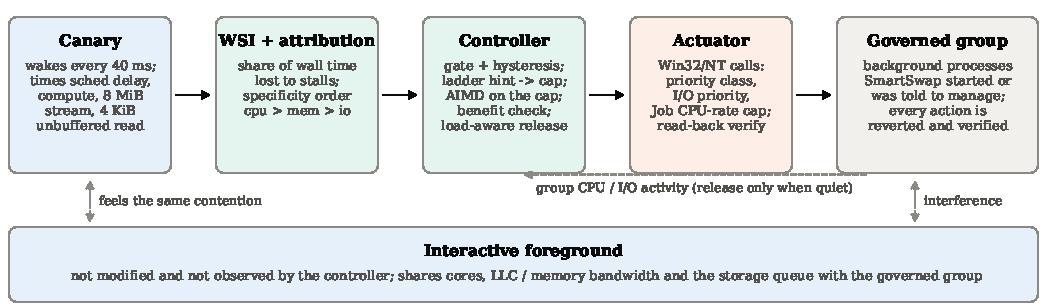
\includegraphics[width=\textwidth]{figures/fig_architecture.pdf}
  \caption{SmartSwap~v2. The controller never observes the foreground it protects; it reasons only from its own canary and from the activity of the processes it governs.}
  \label{fig:arch}
\end{figure*}

\subsection{Canary and the Windows Stall Index}

The canary is a separate low-duty process that wakes every $T=40$\,ms and times four components of one ``beat'': the scheduling delay $s$ between its deadline and its actual wake-up, a fixed interpreter loop $c$ (time-slice sensitive), a streaming copy $m$ of an 8\,MiB buffer (larger than the per-core L2, so last-level-cache and memory-bandwidth sensitive), and one 4\,KiB unbuffered random read $o$ opened with \texttt{FILE\_FLAG\_NO\_BUFFERING} (storage-queue sensitive; the page cache cannot hide it). On an idle host SmartSwap records the median of each component, $\hat{s},\hat{c},\hat{m},\hat{o}$, and their sum $\hat{\ell}$.

Over a sliding window $W$ of the last eight beats, the WSI is the share of wall time the canary lost to interference:
\begin{equation}
\mathrm{WSI} = 100\cdot\frac{\sum_{i\in W}\max\!\left(0,\; s_i+c_i+m_i+o_i-\hat{\ell}\right)}{|W|\,T}\ \%.
\label{eq:wsi}
\end{equation}
WSI is a user-mode analogue of the Linux PSI ``some'' metric~\cite{weiner2018psi}: PSI counts time in which at least one task is stalled on a resource, using kernel instrumentation; WSI estimates the same quantity by direct experience of a probe task, which needs no privilege and works on any Windows build. The canary is in the spirit of Bubble-Up/Bubble-Flux probes~\cite{mars2011bubbleup,yang2013bubbleflux}, but runs continuously on a desktop rather than profiling co-location offline.

\subsection{Specificity-ordered differential attribution}

Each component's \emph{excess} is its window median relative to its idle median: $e_\mathrm{cpu}=(\tilde{s}-\hat{s})/\hat{\ell}$, $e_\mathrm{mem}=(\tilde{m}-\hat{m})/\hat{m}$, $e_\mathrm{io}=(\tilde{o}-\hat{o})/\hat{o}$. A naive ``largest excess wins'' rule fails in practice. In our pilot runs, memory-bandwidth contention inflated the unbuffered read \emph{more} than the memory stream itself (DMA and the I/O completion path compete for the memory controller), so it would have been misattributed to storage. The signals differ in \emph{specificity}, not just magnitude: scheduling delay rises essentially only under CPU contention; the memory stream slows under bandwidth contention but barely under storage load; the read slows under both storage and bandwidth contention. SmartSwap therefore tests the most specific signal first and reports the first resource whose excess crosses a floor $\theta=1$ (the component is at least twice its idle median):
\begin{equation}
\mathrm{cause} = \text{first } r\in\langle\mathrm{cpu},\mathrm{mem},\mathrm{io}\rangle \text{ with } e_r\ge\theta,\ \text{else } \mathrm{none}.
\end{equation}

\subsection{Least-cost ladder with AIMD and benefit verification}

\textbf{Gating.} The controller runs every 200\,ms. It engages only after the WSI exceeds 5\,\% for two consecutive periods and a cause is named, which suppresses one-off spikes.

\textbf{Level 1: resource-matched hint.} The first action costs the background almost nothing when the foreground is mostly idle: for CPU and memory-bandwidth causes, the governed group's priority class is lowered to \texttt{IDLE\_PRIORITY\_CLASS}; for storage, its I/O priority hint is lowered to \emph{very low} via \texttt{NtSetInformationProcess(ProcessIoPriority)}. Mapping memory-bandwidth contention to a CPU-priority hint is an empirical choice. Bandwidth is not a scheduled resource, yet on our hybrid P/E-core pilot host this hint roughly halved probe p95 at negligible throughput cost. We report the effect and do not claim a mechanism (\S\ref{sec:discussion}).

\textbf{Level 2: AIMD-governed CPU-rate cap.} If the WSI stays above the SLO (3\,\%) for three consecutive periods under level~1, the controller places the group in a Job Object and sets a hard CPU-rate cap (\texttt{JOBOBJECT\_CPU\_RATE\_CONTROL\_INFORMATION}~\cite{msjobobjects}), starting at 50\,\% of machine cycles. The cap is then adapted by additive-increase/multiplicative-decrease~\cite{chiu1989aimd}: $\times0.6$ on an SLO violation (with a two-period hold-off so the window can refill) and $+5$ points per calm period. When it climbs back to 100\,\% it is removed and the ladder returns to level~1.

\textbf{Benefit verification.} SmartSwap verifies every action twice. The actuator re-reads kernel state after each call (priority class, I/O priority, job membership, cap flags and rate) and records whether it matches; this establishes that the action \emph{took effect}. The controller then checks that it \emph{helped}: if the mean WSI over the last five periods has not fallen by at least 30\,\% eight periods after a cap was set, the cap is rolled back as ineffective and not retried for ten seconds. A hard cap duty-cycles a job within each scheduling interval, so it can remove throughput without removing bursty interference; the benefit check stops such caps.

\textbf{Load-aware release.} A calm WSI under mitigation usually means the mitigation works, not that the load has left. Early prototypes that released after a calm hold relapsed immediately and oscillated. SmartSwap knows which processes it governs, so it samples their CPU time and I/O bytes each period and releases hints only once the group is quiet (below 0.1 core and 1\,MB/s). When group activity is unknown, it falls back to a calm hold that doubles after every relapse.

\textbf{Safety.} Actions target only the governed group and never raise priorities. Every action is reverted at disengagement or shutdown, and each revert is verified by read-back. Note that closing a Job Object handle does \emph{not} lift a CPU-rate cap from processes still in the job, so the cap is explicitly cleared and the cleared state is read back.

\section{Implementation}
\label{sec:impl}

SmartSwap is a local FastAPI service with a static web dashboard (Python~3.14, \texttt{ctypes} bindings to \texttt{kernel32} and \texttt{ntdll}; no third-party native code). The controller is a pure decision module with no Win32 calls, so it is unit-tested and can be replayed offline from recorded canary traces. Probe and worker programs avoid Python \texttt{multiprocessing}, for a reason that motivated part of this work (\S\ref{sec:lessons}). Background workers stop together on a named manual-reset event, and they bucket completed work units by 100\,ms of wall time so that throughput can be counted exactly inside the foreground's measurement window.
